%LaTeX Template for short student reports.
% Citations should be in bibtex format and go in references.bib
\documentclass[a4paper, 11pt]{article}
\usepackage[top=3cm, bottom=3cm, left = 2cm, right = 2cm]{geometry} 
\geometry{a4paper} 
\usepackage[utf8]{inputenc}
\usepackage{textcomp}
\usepackage{graphicx} 
\usepackage{amsmath,amsfonts,amssymb,amsthm}  
\usepackage{bm}  
\usepackage[backend=bibtex,style=numeric]{biblatex}  %backend=biber is 'better'
\usepackage[bookmarks,colorlinks,breaklinks]{hyperref}  
%\hypersetup{linkcolor=black,citecolor=black,filecolor=black,urlcolor=black} % black links, for printed output
\usepackage{memhfixc} 
\usepackage{pdfsync}  
\usepackage{fancyhdr}
\usepackage{array}
\usepackage[T1]{fontenc}
\usepackage{booktabs, multirow}
\usepackage[
singlelinecheck=false % <-- important
]{caption}
\usepackage{url}
\newcommand{\Lagr}{\mathcal{L}}
\newcommand{\Real}{\mathbb{R}}
\newcommand{\Natural}{\mathbb{N}}
\newcommand{\tangentvector}[2]{\frac{\partial #1}{\partial #2}}
\newcommand{\innerproduct}[2]{\langle #1, #2 \rangle}

\usepackage{musicography}

\graphicspath{ {./images/} }

\pagestyle{fancy}


\renewcommand{\contentsname}{Rozdziały}
\renewcommand{\figurename}{Grafika}
\newtheorem{theorem}{Theorem}
\theoremstyle{definition}
\newtheorem{definition}{Definition}[section]
\newtheorem{example}{Example}[section]

\captionsetup[table]{name=Tabela}

\title{Manifolds}
%\date{}

\addbibresource{references.bib}

\begin{document}
\maketitle
\hypersetup{linkcolor=black}
\tableofcontents

\section{Topology}
TODO: add

\section{Tangent Space}

\subsection{Definition}
Let $(M, \tau)$ be a $C^k$ differentiable manifold, $(U, \phi)$ chart on $M$ and $p \in U$. 
Let $\gamma_1, \gamma_2: (-1, 1) \rightarrow U$ be two curves such that $\gamma_1(0) = \gamma_2(0) = p$ and $D_{\phi \circ \gamma_1}(x), D_{\phi \circ \gamma_2}(x) \in C^k[(-1, 1), R^n]$. \\
Let \texttildelow T be an equivalence relation on the set of curves meeting the above conditions s.t.
$\gamma_1 \text{\texttildelow} \gamma_2 \iff D_{\phi \circ \gamma_1}(\phi \circ \gamma_1)(0) = D_{\phi \circ \gamma_2}(\phi \circ \gamma_2)(0)$. \\
Finally, a tangent space $T_pM$ is defined as a set of equivalence classes of curves meeting the above conditions. \\
\begin{flalign}
	& [\gamma]_\text{\texttildelow} = \{\gamma': (-1, 1) \rightarrow U \text{ s.t. } \gamma \text{\texttildelow} \gamma' \}  \\
	& T_pM = \{[\gamma]_\text{\texttildelow}: (-1, 1) \rightarrow U, \phi \circ \gamma \in C^k[(-1, 1), \mathbb{R}^n], \gamma(0) = p \}
\end{flalign}
Since $\gamma_1(0) = \gamma_2(0) = p \implies D_{\phi \circ \gamma_1}(0) = D_{\phi \circ \gamma_2}(0) \iff [\gamma_1]_\text{\texttildelow} = [\gamma_2]_\text{\texttildelow}$, it follows that\\
SHOW INDEPENDENCE FROM CHART. \\

\subsection{Operations on tangent space}
To define operations on the elements of $T_pM$, if $(U, \phi)$ is a chart with $p \in U$, one may define a map:

\begin{flalign}
	& h_*: T_pM \rightarrow T_{\phi(p)}\mathbb{R}^n = \mathbb{R}^n, \\
	& h_*([\gamma]_\text{\texttildelow}) := D_{\phi \circ \gamma}(0). \\
\end{flalign}
Note that $D_{\phi \circ \gamma}(0)$ is a well defined $\phi \circ \gamma: \Real \rightarrow \Real^n$. \\
\\
Then the operations on $T_pM$ are defined as follows:
\begin{flalign}
	& \text{for } u, v \in T_pM \text{ and } \lambda \in \mathbb{R} \\
	& u + v := h_*^{-1}( h_*(u) + h_*(v) ), \\
	& \lambda v:= h_*^{-1}(\lambda h_*(v) ). \\
\end{flalign}
\subsubsection{Bijectivity} 
By the definition of a chart, it has to be a homeomorphism (continous, bijective) map.
Thus $T_pM$ is a vector space isomorphic to $\mathbb{R}^n$.

\subsubsection{Basis}
If $B = \{e_1, e_2, .. e_n\}$ is a basis of $\mathbb{R}^n$, then $B_{T_pM} = \{h_*^{-1}(e_1), h_*^{-1}(e_2), .. h_*^{-1}(e_n)\}$ is a basis of $T_pM$.
Basis is often denoted by the following notation:
\begin{flalign}
	& \frac{\partial}{\partial x^i}\text{\texttildelow} := h_*^{-1}(e_i) \\
	& \frac{\partial}{\partial x^i}\text{\texttildelow} \in T_pM
\end{flalign}


\subsection{Cotangent Space}
Let $M$ be a $C^k$ differentiable manifold, $p \in M$. \\
If $T_pM$ is a tangent space, then its dual space $T_p^*M$ is called a cotangent space. \\

\subsubsection{Basis of Cotangent Space}
If $B_{T_pM} = \{b_1, b_2, ..., b_n\}$ is a basis of tangent space, then basis of its dual space $B^*_{T_p^*M} = \{b_1^*, b_2^*, ..., b_n^*\}$ can be found as follows:
\begin{flalign}
	& b_i^* \in \Lagr(T_pM \rightarrow \Real), b_j \in B_{T_pM} \\
	& b_i^* (b_j) := \delta_{ij} =
		\begin{cases}
				1, & \text{if } i=j,\\
				0, & \text{if } i\neq j.
		\end{cases}
\end{flalign}
Consider now a basis of a tangent space $\frac{\partial}{\partial x^i}\text{\texttildelow} := h_*^{-1}(e_i)$. \\
Its dual basis is given by $dx_i: T_xM \rightarrow \Real$, $dx_i(\frac{\partial}{\partial x^j}) := \delta{ij}.

\subsection{Directional Derivative}
Let $M$ be a $C^k$ differentiable manifold, $f: M \rightarrow \Real$ be a smooth map, $p \in M$ and $v \in T_pM$. \\
We define a directional derivative as a map:
\begin{flalign}
	& D_vf: T_pM \rightarrow \Real \\
	& D_vf(w) := w(f) = D_{f(\gamma(t))}(t=0) \text{ where } \gamma: (-1, 1) \rightarrow M \text{ s.t. } \gamma(0) = p, \gamma\text{\texttildelow} = v
\end{flalign}

\subsection{Tangent bundle}
Let $M$ be a $C^k$ differentiable manifold. We define a Tangent bundle as a set consisting of all tangent spaces defined as:
$TM := \bigcup\limits_{p \in M} \{p\} \times T_pM$

\subsection{Differential}

Let $(M_1, \tau_1) (M_2, \tau_2)$, be $C^k$ differentiable manifolds, $f: M_1 \rightarrow M_2$ be a smooth map and $p \in U \in \tau_1$. \\
We define a differential (or pushforward) as a map between tangent spaces as follows:
\begin{flalign}
	& df: T_pM_1 \rightarrow T_{f(p)}M_2 \\
	& df([\gamma]_\text{\texttildelow}) := [f \circ \gamma]\text{\texttildelow} \in T_{f(p)}M_2
\end{flalign}
Note that $[f \circ \gamma]\text{\texttildelow}$ is a equivalence class of all curves $f \circ \gamma: (-1, 1) \rightarrow M_2$, with $(f \circ \gamma)(0) = f(p)$ and $(f \circ \gamma_1) \text{\texttildelow} (f \circ \gamma_2) \iff D_{\psi \circ (f \circ \gamma_1)}(0) = D_{\psi \circ (f \circ \gamma_2)}(0)$, for some $\psi$ being a chart of $M_2$ on neighbourhood of $f(p)$. \\\\

Given that $\{\frac{\partial}{\partial x^i} \}$ is a basis for $T_pM_1$ with each term corresponding to a smooth curve $\gamma_i: (-1, 1) \rightarrow M$, $\gamma_i(0) = p$, i.e $\{\frac{\partial}{\partial x^i} = [\gamma_i]_\text{\texttildelow}\}$, $\{\frac{\partial f}{\partial x^i}  = [f \circ \gamma_i]_\text{\texttildelow} \}$ is a basis for $T_{f(p)} M_2$, and is a dual basis of cotangent space $\{dx_i\}$, with $dx_i(\tangentvector{}{x_j}) = \delta{ij}$, then
\begin{flalign}
	& f(x_1, x_2, \dots x_n) = (f_1, f_2, \dots f_m)\\
	& df: T_pM_1 \rightarrow T_{f(p)}M_2 \\
	& u := \sum_{i}^{n} \lambda_i \tangentvector{}{x^i}, \text{ then a differential is defined as } \\
	& df_p(u) = \sum_{i}^{n} \tangentvector{f}{x^i}(p) dx_i(u) \\
	& df_p(u) = \sum_{i}^{n} \tangentvector{f}{x^i}(p) dx_i \left( \sum_{j}^{n} \lambda_j \tangentvector{}{x^j} \right)\\
	& df_p(u) = \sum_{i}^{n} \tangentvector{f}{x^i}(p) dx_i \left( \lambda_i \tangentvector{}{x^i} \right)\\
	& df_p(u) = \sum_{i}^{n} \lambda_i \tangentvector{f}{x^i}(p) \\
	%& df(v) = D_{\phi \circ \gamma_1}(0)\\
\end{flalign}

\section{Submersion}
Let $M, N$ be manifolds and $f: M \rightarrow N$ be a smooth map. \\
Its pushforward $df: T_pM \rightarrow T_{f(p)}N$ is called an immersion if it is a bijective map. \\

\subsubsection{Natural projection}
Natural projection $\pi: TM \rightarrow M$ is defined as:
$\pi(p, T_pM) := p$

\section{Metric Tensor}
Let M be a $C^k$ differentiable manifold and $p \in M$. \\
A metric tensor $g_p: T_pM \times T_pM \rightarrow \Real$ is a map that is: \\
\begin{itemize}
  \item Bilinear: 
		\begin{itemize}
			\item $g_p(u, \lambda v) = g_p(\lambda u, v) = \lambda g_p(u, v)$,
			\item $g_p(u + w, v) = g_p(u, v) + g_p(w, v)$,
			\item $g_p(u, v + w) = g_p(u, v) + g_p(u, w)$.
		\end{itemize}
  \item Symmetric: $g_p(u, v) = g_p(v, u)$.
  \item Nondegenerate:	$\forall v \in T_pM: v \neq 0 \implies \exists u \in T_pM: g_p(u, v) \neq 0$
  \item If $g_{u, v}: M \rightarrow \Real, \text{ with } g_{u, v}(p) := g_p(u, v)$, then \\
$g_{u, v}$ is a smooth function.
\end{itemize}

\section{Riemann semi-maniofld}
Let $M$ be a $C^k$ smooth manifold and $g_p: T_pM \times T_pM \rightarrow \Real$ be its metric tensor. We say that a tuple $(M, g_p)$ is called a Riemann semi-maniofld. \\
$g_p$ is also called a Riemann Metric.

\subsection{Riemann norm}
For a given metric tensor $g_p$, Riemann norm is defined as $\|\cdot\|: T_pM \rightarrow \Real, \text{ with } \|v\| := \sqrt{g_p(v, v)}$

\subsection{Curve length}
Let $\gamma: (a, b) \subseteq \Real \rightarrow M$ be a parametrized smooth map. \\
We define the length of this curve as: \\
$L(\gamma) := \int_a^b \|[\gamma]_\text{\texttildelow}\| dt = \int_a^b \sqrt{g_p([\gamma]_\text{\texttildelow}, [\gamma]_\text{\texttildelow})} dt$


\section{Exterior Algebra}
\subsection{Alternating bilinear form}
Let $V$ be a vector space over a field $F$. An alternating (or antisymmetric) bilinear form on $V$ is a bilinear form $B: V \times V \rightarrow F$ such that $B(v, w) = -B(w, v)$.

\subsection{Second exterior power}
Let $V$ be a finite-dimensional vector space over a field $F$ \\
and $V_B = \{ B: V \times V \rightarrow F : B \text{ is alternating bilinear form.} \}$ be a vector space of all alternating bilinear forms.
The second exterior power of $V$, denoted with $\bigwedge\nolimits^2 V$ is a dual space of $V_B$. i.e. $\bigwedge\nolimits^2 V = V_B^*$. Elements of $\bigwedge\nolimits^2 V$ are called 2-vectors.

\subsection{Exterior product}
Let $V$ be a finite-dimensional vector space over a field $F$ and $v, u \in V$ and $\bigwedge\nolimits^2 V$ be its second exterior power. Exterior product of $v$ and $u$, is a linear map to $F$ $v \wedge u \in \bigwedge\nolimits^2 V$ \\
$(v \wedge u)(B) = B(v, u)$. \\\\
From this definition, the following properties follow:
\begin{flalign}
	&(u \wedge v)(B) = B(u, v) = -(u \wedge v)(B) = -B(v, u) \\
	&(u \wedge u)(B) = -(u \wedge u)(B) = 0 \\
	&\text{if $\{v_1, v_2, \dots, v_n\}$ is a basis for $V$, then $\{ v_i \wedge v_j: i, j \in \{1, 2, \dots, n\}, i < j \}$ is a basis for $\bigwedge\nolimits^2 V$.}
\end{flalign}

\begin{theorem}
	$u, v \in V, u \neq 0 \implies (u \wedge v = 0 \iff \exists_{\lambda \in F}: v = \lambda u)$
	\begin{proof}
	This basically mean that $u, v$ are in the same subspace and this may be shown with the following. \\
	Let $v = \lambda u$. Then $u \wedge v = u \wedge (\lambda u) = \lambda (u \wedge u) = 0$. \\
	\end{proof}
\end{theorem}

\subsection{Alternating multilinear form}
\begin{definition}
Let $V$ be a vector space over field $F$. An alternating multilinear form of degree $p$ is a map: $V \times V \times \dots \times V \rightarrow F$ such that

\begin{flalign}
&M(u_1, \dots, u_i, \dots, u_j, \dots u_p) = M(u_1, \dots, u_j, \dots, u_i, \dots u_p) \\
&M(u_1,\dots, \lambda u_i + w, \dots, \dots u_p) = \lambda M(u_1, \dots, u_i, \dots, \dots u_p) + M(u_1, \dots, w, \dots, \dots u_p)
\end{flalign}
The set of all such forms $M$ is a vector space. Let $a_i: \{0, \dots, p\} \rightarrow \{0, \dots, n\}$ be a strictly increasing sequence, and $\{v_1, \dots, v_n\}$ be a basis of $V$. Then a multilinear form $M$ of degree $p$ for any set of vectors in a given basis can be trivially transformed by the properties of $M$ into a form $M(u_1, \dots u_2) = \lambda_1 M(v_{a_1}, \dots v_{a_p}) + \lambda_2 M(v_{a_1}, \dots v_{a_p}) + \dots, 
$M(v_{a_1}, \dots, v_{a_p})$. Since $a_i$ is strictly increasing, if we choose $p$ elements out of $n$, there are ${n}\choose{p}$ possibilities to do it. ${n}\choose{p}$ is also a dimension of the vector space of such forms $M$. In particular, if $p > n$, we just define a dimension to be 0.

\begin{example}
Let 
\[
A = 
\begin{bmatrix}
    v_1 & v_2 & \dots & v_n \\
\end{bmatrix}
\] be a matrix in $\Real^n$.\\
Then a map $M(v_1, v_2, \dots, v_n) = det(A)$ is an alternating multilinear form of degree $n$.
\end{example}

\end{definition}

\subsection{Dual Operator}
\begin{definition}
Let $X, Y$ be normed vector spaces and $T: X \rightarrow Y$ be a linear operator. Dual operator $T^*: Y^* \rightarrow X^*$ (note the reversed $Y^*, X^*$) is defined as $T^*(f) = f \circ T$.
\end{definition}

\subsection{p-th exterior power}
\begin{definition}
	Let $V$ be a finite-dimensional vector space over field $F$, \\
	and $V_{AM} = \{ B: V \times \dots \times V \rightarrow F : B \text{ is alternating multilinear form.} \}$ be a vector space of all alternating multilinear forms over $V$. p-th exterior power of $V$, denoted with $\bigwedge\nolimits^p V$ is a dual space of $V_{AM}$. i.e. $\bigwedge\nolimits^p V = V_{AM}^*$. Elements of $\bigwedge\nolimits^p V$ are called p-vectors.
\end{definition}

\begin{definition}
	Given $u_1, u_2 \dots, u_n \in V$, the exterior product is a linear map \\
	$u_1 \wedge u_2 \wedge \dots \wedge u_n: V_{AM} \rightarrow F$ such that $(u_1 \wedge u_2 \wedge \dots \wedge u_n)(M) = M(u_1, u_2, \dots u_n)$.
\end{definition}

\begin{theorem}
$u_1 \wedge u_2 \wedge \dots \wedge u_n = 0 \iff \\
(\exists \lambda_1, \lambda_2, \dots \lambda_n \in F: \exists i \in \{1, \dots, n\}: \lambda_i \neq 0: 
\lambda_1 u_1 + \lambda_2 u_2 \dots + \lambda_n u_n = 0 \text{ i.e. they are linearly dependent} )$
\begin{proof}
Without a loss of generality assume that $u_n = \lambda_1 u_1 + \lambda_2 u_2 \dots$ \\
Then due to definition based on alternating multilinear forms, it follows that \\
$M(u_1, u_2, \dots, u_n) = M(u_1, u_2, \dots, \lambda_1 u_1 + \lambda_2 u_2 \dots) = \\ 
\lambda_1 M(u_1, u_2, \dots, u_1) + \lambda_2 M(u_1, u_2, \dots, u_2) + \dots = \\
\text{(by the antilinear property, swapping for each element a pair)} (u_i, u_{n-i}),  \\
= -\lambda_1 M(u_1, u_2, \dots, u_1) -\lambda_2 M(u_1, u_2, \dots, u_2) -\dots$ \\
Finishing with $a = -a \iff a = 0$
\end{proof}
\end{theorem}

Exterior powers have natural properties w.r.t. the linear transformations. Given a linear operator $T: V \rightarrow W$ and a form $M: W \times W \times \dots \times W \rightarrow F_W$, we may induce an operator \\
$T^*M: V \times V \dots \times V \rightarrow F_W$ as $(T^*M)(v_1, v_2, \dots, v_n) := M(T v_1, T v_2, \dots T v_n)$.
\\\\
This defines a dual map $\bigwedge^p T: \bigwedge^p V \rightarrow \bigwedge^p W$, $(\bigwedge^p T)(v_1 \wedge v_2 \dots) := (T v_1) \wedge (T v_2) \dots$

\begin{example}
One of such maps is very familiar and used frequently. Take $p = n$ for some $n$-dimensional vector space $V$. Then a vector space $\bigwedge^pV$ is 1 dimensional as ${n}\choose{p}$ = ${n}\choose{n}$ = 1 and the dimension of a dual space of all the alternating linear forms, $V^*_{AL}$ is equal to the dimension of the vector space $V_{AL}$ itself.
In fact, this map is a determinant itself. \\
Observe that $\bigwedge^n(v_1 \wedge \dots \wedge v_n) = T v_1 \wedge \dots \wedge Tv_n$, ... TODO
\end{example}

\section{differential forms}

\subsection{1-forms}
\begin{definition}
Let $M_1, M_2$ be a n-dimensional, $C^k$ smooth manifolds and $x \in M$. \\
We define a 1-form mapping $\omega_x: T_xM \rightarrow \Real$, where $\omega_x(u)$ is a linear form. \\
Vector space of such 1-forms is isomorphic to a vector space $\bigwedge^1(T_xM)$.

\end{definition}
\begin{example}
	Consider a tangent space $T_xM$ with a basis $\frac{\partial}{\partial x^i}$ and its dual basis $dx_i(\tangentvector{}{x^j}) := \delta{ij}$.
	Let $\omega: T_xM \rightarrow \Real$, $\omega(u) = f(u) dx_1(u)$. Given that $u = \sum_{n}^{i=1} \lambda_i \tangentvector{}{x^i}$, it follows that
	\begin{flalign}
		&\omega(u) = f(u) dx_1 \left(\sum_{n}^{i=1} \lambda_i \tangentvector{}{x^i}\right). \text{ Then it follows, that from linearity of $w, dx_1$ }\\
		&\omega(u) = f(u) \sum_{n}^{i=1} \left(\lambda_i dx_1\left(\tangentvector{}{x^i}\right)\right) \\
		&\omega(u) = f(u) \sum_{n}^{i=1} \lambda_i \delta_{i, 1} \text{, and finally } \\
		&\omega(u) = f(u) \lambda_1
	\end{flalign}
\end{example}

\subsection{Basis of a vector space of 1-forms, $\bigwedge^1(T_xM)$}
%Given a smooth function $f: M_1 \rightarrow M_2$, we define its exterior derivative as:
%$df(u) := \sum_{n}^{i=1} \tangentvector{f}{x^i} dx_i(u)$. $df$ is a vector in $\bigwedge^1(T_xM)$.

\subsection{k-form}
%\subsubsection{notation}
%From now on, any p-vector of form $dx_{i_1} \wedge dx_{i_2} \wedge \dots \wedge dx_{i_k}$ for $I = \{i_1, i_2, \dots i_n\}$ being a strictly increasing sequence, will be denoted with $dx_{123\dots k}$. Simirarly if $k=3$, we will denote $dx := 
\begin{definition}
	Given a vector $\omega \in \bigwedge^n(TxM)$, with $\omega = \sum \tangentvector{f}{x^i}$ 
\end{definition}

\section{Integration of differential forms}

\subsection{Integration of 1-forms}
\begin{definition}
\end{definition}

\section{Tensor Space}
\begin{definition}
	Let $\{V_i\}$ be a set of vector spaces. The map $\tau: \prod V_i \rightarrow F$, where $F$ is some common field for all the vector spaces, is called k-linear if its linear in each component. Set of all such maps form a vector space.
\end{definition}
\begin{definition}
	Let now $V_i = V$. We define $T^k(V) := \{\tau: \prod^k V \rightarrow F$, \tau - \text{multilinear} \}$ 
\end{definition}
Let us consider $T^1(V)$. $\tau \in T^1(V)$ takes $1$ copy of $V$. 
$\tau: V \rightarrow F$. Since $\tau$ is linear in its only argument, the vector space of all such functions is simply a dual space of $V$. We may understand $T^k(V)$ as a generalization of dual space to product spaces.

\begin{theorem}
	Let $T \in L(V, W)$ (L - set of all linear op. from V to W), then
	$\exists T^*: \tau^k(W) \rightarrow \tau^k(V)$
\end{theorem}

\begin{definition}
	Let $\tau \in T^k(V), \sigma \in T^l(V)$. We define their tensor product as follows:
	$\tau \otimes \sigma \in T^{k+l}$,  \\
	$\tau \otimes \sigma(v_1, \dots, v_k, v_{k+1}, \dots, v_{k+l}) = \tau(v_1, \dots, v_k)\sigma(v_{k+1}, \dots, v_{k+l})$
\end{definition}

This definition yields 2 facts: \\
$\tau \otimes \sigma \neq \sigma \otimes \tau$ - non commutative. \\
$(\tau \otimes \sigma) \otimes \omega = \tau \otimes (\sigma \otimes \omega)$ - associative

\subsection{Tensor Product}
Let $V$, $W$ be two vector spaces. We define a tensor product as a vector space $A$ with a bilinear map $f: V \times W \rightarrow A$ with so called universal property. i.e. given a vector space $Z$ and a bilinear map $\tau: V \times W \rightarrow Z$, $\exists! \bar{\tau}: A \rightarrow Z: \bar{\tau} \circ f = \tau$. Usually in this context $A$ and $f$ are denoted by $V \otimes W := A$ and $\otimes := f$.
\begin{figure}[h]
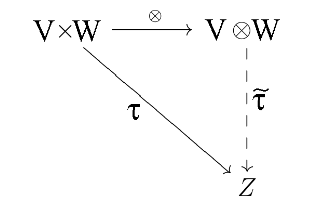
\includegraphics{universal_property}
\caption{Universal property}
\end{figure}

\begin{theorem}
	Tensor product between 2 vector spaces always exists.
	\begin{proof}
		TODO
	\end{proof}
\end{theorem}

\subsection{Tensor basis}
Given 2 vector spaces $V, W$ and their bases $B_V, B_W$, they induce a basis for $V \otimes W$ as follows:
$B_V \otimes B_W = \{v_i \otimes w_j, \text{ where } $v_i \in B_V, w_j \in B_W\}$, . Thus it has $\dim(V) \dim(W)$ elements. \\
i.e. $V \otimes W \cong \mathbb{R}^{\dim(V) \dim(W)}$.
\subsubsection{Simple Tensors}
Now given these bases and a scalar $a \in F$, we can define a simple tensor as $a (v_i \otimes w_j)$. \\
Given any tensor $T \in V \otimes W$, we can write it as a linear combination of simple tensors. \\
$T = \sum_{i, j} a_{ij} v_i \otimes w_j$ for some $a_{ij} \in F$.
Following properties of tensor product follow:
\begin{flalign*}
	& (v_1 + v_2) \otimes w = v_1 \otimes w + v_2 \otimes w \\
	& v \otimes (w_1 + w_2) = v \otimes w_1 + v \otimes w_2 \\
	& (a v) \otimes w = v \otimes (a w) = a (v \otimes w)
\end{flalign*}

\subsection{Tensor type (n, k)}
\begin{definition}
	Let $V$ be a vector space. We define a tensor type $(n, k)$ as a tensor product of $n$ copies of $V$ and $k$ copies of $V^*$. 
	$T^n_k(V) := V \otimes \dots \otimes V \otimes V^* \otimes \dots \otimes V^*$.	\\
\end{definition}
\subsubsection{Tensor product between type (n, k) and (m, l)}
Earlier we defined how to multiply 2 tensors $\tau \in T^k(V) = T^k_0(V), \sigma \in T^l(V) = T^l_0(V)$, which correspond to the tensor types $(k, 0)$ and $(l, 0)$ respectively. i.e.
\begin{flalign}
	&\tau \otimes \sigma \in T^{k+l},  \\
	&\tau \otimes \sigma(v_1, \dots, v_k, v_{k+1}, \dots, v_{k+l}) = \tau(v_1, \dots, v_k)\sigma(v_{k+1}, \dots, v_{k+l})
\end{flalign}
We can generalize this to any tensors of types (n, k), (m, l) as follows:
\begin{flalign}
	&\tau \in T^n_k(V), \sigma \in T^m_l(V) \\
	&\tau \otimes \sigma \in T^{n+m}_{k+l}(V) \\
	&(\tau \otimes \sigma)^{i_1 \dots i_{n+m}}_{j_1 \dots j_{k+l}} = \tau^{i_1 \dots i_n}_{j_1 \dots j_k} \sigma^{i_{n+1} \dots i_{n+m}}_{j_{k+1} \dots j_{k+l}}
\end{flalign}


\begin{example}
	$T^0_0$ is a scalar,	       								\\
	$T^1_0$ is a vector,    	   								\\
	$T^0_1$ is a covector, linear functionals, 1-forms	 		\\
	$T^1_1$ is a linear map,	 								\\
\end{example}
\begin{example}
	An inner produce, a 2-form (or bilinear form) is a tensor of type $(0, 2)$. \\
	A bivector is a tensor of type $(2, 0)$. \\
	If dim(V) = 3, then a cross product is an example of a (1, 2) tensor.

\end{example}

\subsection{Einstein summation}
To abbreviate summing over all the elements in an expression such as $a = \sum_i {x_i f_i}$, we may use Einstein notation. That is, unless stated otherwise we implicitly assume that an expression $\sum_i {x_i f_i}$, may be abbreviated to skip the summation just to $x_i f_i$. Then $a = x_i f_i$.

\newpage

\subsection{Covariant/contravariant transformations}
Let $f = (X_1, X_2, \dots, Y_n)^T$, $\tilde{f} = (Y_1, Y_2, \dots, Y_n)^T$, $n \in \Natural$ be bases of some vector space $V$.
Then any vector $v \in V$ can be uniquely expressed as a linear combination of these bases. Change of basis is given by:
\begin{flalign} 
& f = (X_1, \dots, X_n) \rightarrow \tilde{f} = (\sum_i{a_j^1 X_j}, \dots, \sum_i{a_j^n X_j}) = (Y_1, \dots, Y_n) \\
\iff \\
& fA = \tilde{f} \label{eq:covectors_basis_invariance}
\end{flalign}
for some change of basis matrix $A \in M_{\Real^n \times \Real^n}$, with $A_{ij} = a^i_j$ i.e. superscript describing the row.
That is, $Y_j = \sum_i{a_i^j X_j}$.
We may denote a vector $v$ in a basis $f$ as a vector 
\begin{flalign} \label{eq_contravariant_basis}
	[v]_f = (v^1, \dots v^n)^T_f,
\end{flalign}
which elements may be referenced by $[v]_f^i = v^i$. \textbf{$v^i$ is only valid in this context!}

By \ref{eq_contravariant_basis}, it follows that $v$ may be written as a matrix product:
\begin{flalign}
	v = (X_1, \dots, X_n) (v^1, \dots v^n)^T_f = f [v]_f
\end{flalign}
Similarly we may do exactly the same for the basis $\tilde{f}$.
\begin{flalign}
	v = (Y_1, \dots, Y_n) (v^1, \dots v^n)^T_{\tilde{f}} = \tilde{f} [v]_{\tilde{f}}
\end{flalign}
Combining these 2, yields
\begin{flalign}
	&v = f [v]_f = \tilde{f} [v]_{\tilde{f}}. \\
\end{flalign}
By relation \ref{eq:covectors_basis_invariance}, we have
\begin{flalign}
	v = f [v]_f = \tilde{f} [v]_{\tilde{f}}. \iff 
	v = f [v]_f = fA [v]_{\tilde{f}}. 
\end{flalign}
Assuming that $f \neq 0$, 
\begin{flalign}
	[v]_f = A [v]_{\tilde{f}}. 
\end{flalign}
Since $A$ is invertible, we may claim that
\begin{flalign}
	A^{-1}[v]_f = [v]_{\tilde{f}}. 
\end{flalign}
Now we may denote $A^{-1}_{ij} = \tilde{a}^i_j$, and finally applying multiplication to each row
\begin{flalign}
	\sum_{j} \tilde{a}^i_j [v]_f^j = [v]_{\tilde{f}}^i,
\end{flalign}
i.e. i-th row of $A^{-1}$ dotted with $[v]_f$.
\begin{definition}
	Because change of basis from $[v]_f$ to $[v]_{\tilde{f}}$ transform with the inverse of $A$, $A^{-1}$, we say that components of $[v]_f$ to $[v]_{\tilde{f}}$ transform contravariantly.
\end{definition}



\section{Musical isomorphisms}
Let $TM$ be a tangent bundle, $T^*M$ be a cotangent bundle and $\innerproduct{.}{.}: TM \times TM$ be an inner product. We define a musical isomorphisms $\musFlat{}: TM \rightarrow T^*M$ s.t. $\forall x, y \in TM: x^{\musFlat{}}(y) = \innerproduct{x}{y}$ \\
Similarly its inverse is expressed by the operator $\musSharp: T^*M \rightarrow TM$ s.t. $\forall \omega \in T^*M, \forall y \in TM: x(y) = \innerproduct{x^{\musSharp}}{y}$


\end{document}

